\section*{Results}
\subsection{Robotic Platforms and surveys }
 \rpsm{Task to: Renato}

in this topic we can describe the results in terms of experimental settings of the multiple robots used to localize the front and study it at different scales with results on the surveys performed from different assets). Here the results can be presented in a way that shows how our approach was able to provide a \emph{cascade of results} that goes from a large scale to mesoscale and then sub-mesoscale understanding of the oceanographic feature. 
We can also mention the difficulties in localizing this feature and highlight what was necessary to gather in terms of assets and data as well as coordination/network to accomplish this first objective.\\

\begin{figure}
    \centering
    \missingfigure[figwidth=0.7\textwidth]{Figure that show somehow results obtained from the different settings producing large scale (identify and localize the front) and mesoscale (identify and localize the front jet) results (we can probably include an A and B figures \cmag{Perhaps we can dedicate this figure just to show the results obtained in terms of capacity in locating and identifying the front on a large scale (with the use of gliders, RV, satellites, command of operations on land, etc. figure 3A) and another that shows results in terms of the filament location and identification (mesoscale) (Figure 3B, AUVs, RV, CTDs, etc.)}}
    \label{fig:block}
\end{figure}

\subsection{Hydrodrography of mesoscale STF phenomena}
\rpsm{Task to: Francisco and hydrodynamic working group}

here we can show the results obtained from the network approach used to study the hydrodynamics of the filament, we can show data from the multiple assets used that provide the development the hydrodynamic model of this mesoscale feature inside the STF). Basically we can include here the general results that are coming out from the Hydrodynamic analysis group. 
The FSLE results could be included in this section in order to relate the in situ identification of the jet and satellite results.\\

\begin{figure}
    \centering
    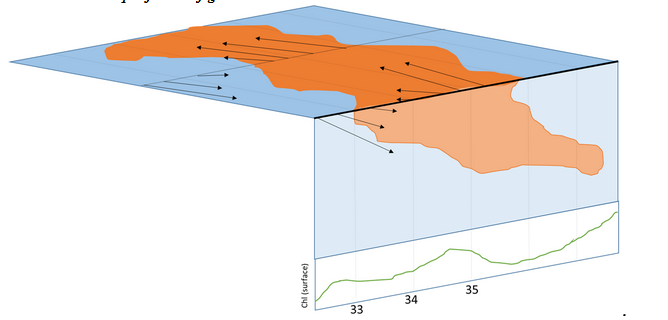
\includegraphics[width=1\linewidth]{figs/3d_results.png}
    \caption{THIS IS A SCHEMATIC EXAMPLE: Meso/submesoscale results from jet hydrodynamic model from zoom area analysis. it will be nice to have a 3D figure. check fig 2 and 4 of this \href{https://journals.ametsoc.org/view/journals/bams/101/11/bamsD190305.xml?tab_body=fulltext-display}{\textbf{paper}}}
    \label{fig:block}
\end{figure}

\subsection{Integration of mesoscale biological and biogeochemical dynamics}
\rpsm{Task to: Catarina and Javier} 
\icomnt{novelty in way to choose the plasce where to sample in terms biology (rosete and other assets)}

here we can show the results obtained in terms of biological (chla, microbial communities) and biogeochemical (nutrients, oxygen, pH) distribution in the zoom area and how the dynamics of the biological and biogeochemical compartment is linked to the hydrodynamics of these kind of mesoscale features.  Basically we can include here the biological and biogeochemical results presented in our previous meetings linked with the physical forces. 
Highlight the research potential of the engagement of researchers with different backgrounds in the decisions. Using different assets, there is a possibility to explore secondary interests that come during the cruise. \\

\begin{figure}
    \centering
    \missingfigure[figwidth=0.7\textwidth]{Results showing how our approach was able to link biological/ biogeochemical/ dynamics and physical forces in the zoom area}
    \label{fig:block}
\end{figure}